% !TEX TS-program = XeLaTeX
% use the following command:
% all document files must be coded in UTF-8
\documentclass[portuguese]{textolivre}
% build HTML with: make4ht -e build.lua -c textolivre.cfg -x -u article "fn-in,svg,pic-align"

\journalname{Texto Livre}
\thevolume{15}
%\thenumber{1} % old template
\theyear{2022}
\receiveddate{\DTMdisplaydate{2021}{8}{20}{-1}} % YYYY MM DD
\accepteddate{\DTMdisplaydate{2021}{10}{26}{-1}}
\publisheddate{\DTMdisplaydate{2021}{11}{19}{-1}}
\corrauthor{Valesca Brasil Irala}
\articledoi{10.35699/1983-3652.2022.35747}
%\articleid{NNNN} % if the article ID is not the last 5 numbers of its DOI, provide it using \articleid{} commmand
% list of available sesscions in the journal: articles, dossier, reports, essays, reviews, interviews
\articlesessionname{articles}
\runningauthor{Ortega e Irala} 
%\editorname{Leonardo Araújo} % old template
\sectioneditorname{Daniervelin Pereira}
\layouteditorname{Anna Izabella Pereira}

\title{Mensuração do engajamento \textit{online} de estudantes do ensino superior: uma revisão de escopo na literatura internacional}
\othertitle{The measurement of student online engagement of higher education: a scoping review in the international literature}
% if there is a third language title, add here:
%\othertitle{Artikelvorlage zur Einreichung beim Texto Livre Journal}

\author[1]{Fernanda da Cunha Ortega \orcid{0000-0002-3361-029X} \thanks{Email: \url{fernandaortega@unipampa.edu.br}}}
\author[1]{Valesca Brasil Irala \orcid{0000-0001-6190-8440} \thanks{Email: \url{valescairala@unipampa.edu.br}}}
\affil[1]{Universidade Federal do Pampa, Departamento de Educação, Bagé, RS, Brasil.}

\addbibresource{article.bib}
% use biber instead of bibtex
% $ biber article

% used to create dummy text for the template file
\definecolor{dark-gray}{gray}{0.35} % color used to display dummy texts
\usepackage{lipsum}
\SetLipsumParListSurrounders{\colorlet{oldcolor}{.}\color{dark-gray}}{\color{oldcolor}}

% used here only to provide the XeLaTeX and BibTeX logos
\usepackage{hologo}

% if you use multirows in a table, include the multirow package
\usepackage{multirow}

% provides sidewaysfigure environment
\usepackage{rotating}

% CUSTOM EPIGRAPH - BEGIN 
%%% https://tex.stackexchange.com/questions/193178/specific-epigraph-style
\usepackage{epigraph}
\renewcommand\textflush{flushright}
\makeatletter
\newlength\epitextskip
\pretocmd{\@epitext}{\em}{}{}
\apptocmd{\@epitext}{\em}{}{}
\patchcmd{\epigraph}{\@epitext{#1}\\}{\@epitext{#1}\\[\epitextskip]}{}{}
\makeatother
\setlength\epigraphrule{0pt}
\setlength\epitextskip{0.5ex}
\setlength\epigraphwidth{.7\textwidth}
% CUSTOM EPIGRAPH - END

% LANGUAGE - BEGIN
% ARABIC
% for languages that use special fonts, you must provide the typeface that will be used
% \setotherlanguage{arabic}
% \newfontfamily\arabicfont[Script=Arabic]{Amiri}
% \newfontfamily\arabicfontsf[Script=Arabic]{Amiri}
% \newfontfamily\arabicfonttt[Script=Arabic]{Amiri}
%
% in the article, to add arabic text use: \textlang{arabic}{ ... }
%
% RUSSIAN
% for russian text we also need to define fonts with support for Cyrillic script
% \usepackage{fontspec}
% \setotherlanguage{russian}
% \newfontfamily\cyrillicfont{Times New Roman}
% \newfontfamily\cyrillicfontsf{Times New Roman}[Script=Cyrillic]
% \newfontfamily\cyrillicfonttt{Times New Roman}[Script=Cyrillic]
%
% in the text use \begin{russian} ... \end{russian}
% LANGUAGE - END

% EMOJIS - BEGIN
% to use emoticons in your manuscript
% https://stackoverflow.com/questions/190145/how-to-insert-emoticons-in-latex/57076064
% using font Symbola, which has full support
% the font may be downloaded at:
% https://dn-works.com/ufas/
% add to preamble:
% \newfontfamily\Symbola{Symbola}
% in the text use:
% {\Symbola }
% EMOJIS - END

% LABEL REFERENCE TO DESCRIPTIVE LIST - BEGIN
% reference itens in a descriptive list using their labels instead of numbers
% insert the code below in the preambule:
%\makeatletter
%\let\orgdescriptionlabel\descriptionlabel
%\renewcommand*{\descriptionlabel}[1]{%
%  \let\orglabel\label
%  \let\label\@gobble
%  \phantomsection
%  \edef\@currentlabel{#1\unskip}%
%  \let\label\orglabel
%  \orgdescriptionlabel{#1}%
%}
%\makeatother
%
% in your document, use as illustraded here:
%\begin{description}
%  \item[first\label{itm1}] this is only an example;
%  % ...  add more items
%\end{description}
% LABEL REFERENCE TO DESCRIPTIVE LIST - END


% add line numbers for submission
%\usepackage{lineno}
%\linenumbers

\begin{document}
\maketitle

\begin{polyabstract}
\begin{abstract}
Este artigo é uma revisão de escopo que tem o objetivo de identificar os instrumentos de coleta e de análise da mensuração do engajamento \textit{online} utilizados em pesquisas internacionais, visando à escolha para utilização escalonável e adaptação ao Ensino Superior brasileiro. A pesquisa foi realizada na base de dados Dimensions, no período de 2017 a 2021. A quantidade de documentos obtidos foi de 162, que, após a etapa de triagem, resultou em uma amostra de dez artigos. Os instrumentos são contextualizados no ensino superior e os quatro mais atuais foram desenvolvidos no período de pandemia da Covid-19. A maioria dos artigos é de abordagem quantitativa e todos utilizam algum tipo de questionário de autorrelato para coletar dados, que são, em maior número, de perguntas fechadas e de escala Likert de 5 pontos. A técnica de análise que mais se repete nos artigos é a modelagem de equações estruturais. Dos dez questionários avaliados, concluímos que o de \textcite{sun2012} é o que melhor atende aos critérios para avaliação do engajamento \textit{online} do estudante no contexto do ensino superior, ao trazer em seus elementos uma configuração passível de ser escalonável para diferentes contextos institucionais e abrangência de disciplinas.

\keywords{Engajamento online \sep Engajamento do aluno \sep Ensino superior \sep Autorrelato}
\end{abstract}

\begin{english}
\begin{abstract}
This article is a scope review  whose main goal is to identify the instruments for collecting and analyzing the measurement of online engagement used in international research,  aiming at the choice for scalable use and adaptation to Brazilian Higher Education. Dimensions database was searched from 2017 to 2021.  There was a total of 162 obtained documents, which after the screening resulted in a sample of 10 articles. The context for using these instruments is higher education and the four most recent ones were developed during the Covid-19 pandemic period. Most articles have a quantitative approach. All use some type of self-report questionnaire to collect data, which mostly consist of questions and a 5-point Likert scale.  The most repeated analysis technique in the articles is structural equation modeling. Of the ten selected questionnaires, we conclude that the one by Sun and Rueda (2012) is the one that best provides the criteria for analyzing student online engagement in the context of higher education, by bringing in its elements a configuration that can be scalable to different institutional contexts and  a wide range of disciplines.

\keywords{Online engagement \sep Student engagement \sep Higher education \sep Self-report}
\end{abstract}
\end{english}
% if there is another abstract, insert it here using the same scheme
\end{polyabstract}

\section{Introdução}\label{sec-intro}
O ano de 2020, com a chegada da pandemia de covid-19, apresentou ao mundo uma nova realidade no ensino, o que provocou uma mudança profunda nas dinâmicas institucionais. Depois da interrupção das atividades presenciais, professores e alunos migraram integralmente para as aulas online. Esse ambiente online, que era anteriormente utilizado somente como apoio no aprendizado para grande parte dos docentes e estudantes dos cursos presenciais, tornou-se imediatamente uma ferramenta essencial e indispensável para a continuidade dos processos de ensino-aprendizagem.

Em vista disso, há uma grande relevância em se pensar no constructo teórico de engajamento dos estudantes no aprendizado online, inclusive a médio e longo prazos, quando se mostram intensificadas as demandas por modelos híbridos \cite{horn2015}. O engajamento do aluno no ensino superior é uma área que tem ganhado grande destaque nos últimos anos, por ser considerado uma variável que pode influenciar o desempenho dos estudantes, intervindo no êxito para conclusão dos estudos \cite{redmond2018}. O engajamento tem uma forte relação com o aprendizado e a satisfação dos estudantes e tem se mostrado como uma tendência de pesquisas mundiais, com inúmeros estudos focados nas mais diversas perspectivas teóricas e metodológicas \cite{hu2012}. No contexto da pandemia da Covid-19, o conceito de engajamento online se tornou uma variável de interesse ainda mais relevante, permeada por diversos aspectos a serem observados, os quais não seriam totalmente idênticos aos analisados em um modelo apenas de ensino presencial \cite{wang2021, heidari2021, shah2021}.

Considerando o crescimento em relação às pesquisas direcionadas ao tema engajamento online mencionado anteriormente, avaliamos, no âmbito do projeto de pesquisa intitulado “Aprendizagens ativas e colaborativas: análise da percepção docente, engajamento discente, da autorregulação e do processo avaliativo” e ao Grupo de Pesquisa sobre Aprendizagens, Metodologias e Avaliação (GAMA), ser pertinente identificar os instrumentos e as técnicas analíticas que estão sendo utilizadas atualmente para mensurar o engajamento online dos estudantes no ensino superior em âmbito internacional, de modo a compará-los e, posteriormente, realizar a sua adaptação e utilização escalonável para o contexto nacional.

Assim sendo, este artigo propõem uma revisão de escopo \cite{tricco2018}, pois consideramos que a natureza desse modelo é adequada ao objetivo geral desta pesquisa, que visa mapear os instrumentos de coleta e de análise da mensuração do engajamento online validados pela literatura internacional, examinando-os comparativamente. A pergunta central norteadora é, portanto, a seguinte: quais são as características dos instrumentos e das técnicas analíticas utilizadas para a mensuração do engajamento online de estudantes do Ensino Superior em pesquisas publicadas recentemente (2017-2021) na literatura internacional? A pesquisa tem como foco a produção de artigos de acesso aberto, publicados entre os anos de 2017 a 2020, os quais possuem como tema central o engajamento online dos estudantes de ensino superior.

Com esse mapeamento, buscamos contribuir sobretudo para a análise descritivo-comparativa a respeito dos diferentes instrumentos de pesquisa já utilizados pela literatura internacional, que focam no engajamento online do estudante, o que cada um deles pode oferecer, a que tipo de pesquisa se prestam e, porventura, quais podem ser preferíveis no contexto nacional. Ademais, vale destacar que no Brasil não foi localizada uma revisão de escopo que apresente este mesmo objetivo. Nesse sentido, consideramos ser de grande relevância aos estudiosos do tema a revisão efetuada.

\section{Definindo o engajamento online}
O construto engajamento estudantil vem sendo pesquisado desde os anos 1930, ainda que rotulado por terminologias diversas que permearam a evolução do conceito \cite{rigo2018}. Também, é um construto que tem se mostrado como foco de interesse das mais diversas áreas do conhecimento \cite{irala2020}. O uso popularizado de um instrumento intitulado \emph{National Survey of Studant Engagement} (NSSE), desenvolvido no contexto norte-americano, impulsionou a consolidação do engajamento dos estudantes no léxico das políticas para o ensino superior \cite{kuh2009}, expandindo-se para outros países de língua inglesa e, nos últimos anos, estendendo-se a diversos outros países.

Atualmente, pesquisas sobre os padrões de engajamento dos estudantes em ambientes online vêm sendo conduzidas, considerando a grande popularização dessas experiências de aprendizagem, seja no ensino presencial, seja no ensino a distância. Ainda, recentemente, têm se mostrado como uma tendência os modelos denominados híbridos, definidos como “qualquer programa educacional formal, no qual o estudante aprende, pelo menos em parte, por meio do ensino online” \cite[p. 34]{horn2015}.

Com a expansão da aprendizagem online, surge um novo âmbito de interesse para empreender as análises sobre o engajamento do estudante: o engajamento online. O engajamento do aluno no aprendizado online é um indicador relevante para a avaliação da aprendizagem dos estudantes, onde seu nível de engajamento é um prognóstico do êxito na aprendizagem \cite{hu2017}. Pode ainda, ser vinculado à dedicação e a energia entregue pelo estudante dentro da sua comunidade de aprendizagem, sendo composto por uma série de condições internas e estruturais, como a aprendizagem de atividades, o ambiente de aprendizagem e as complexas relações interpessoais. Quanto mais engajado está o estudante, maior a possibilidade de direcionar essa energia para o seu aprendizado, o que pode levar a resultados que ampliam ainda mais seus níveis de engajamento \cite{bond2019}. Com o objetivo de sintetizar as dimensões do engajamento online consideradas pelos autores aqui citados, foi construída a \Cref{fig1}.

\begin{figure}[htbp]
 \centering
 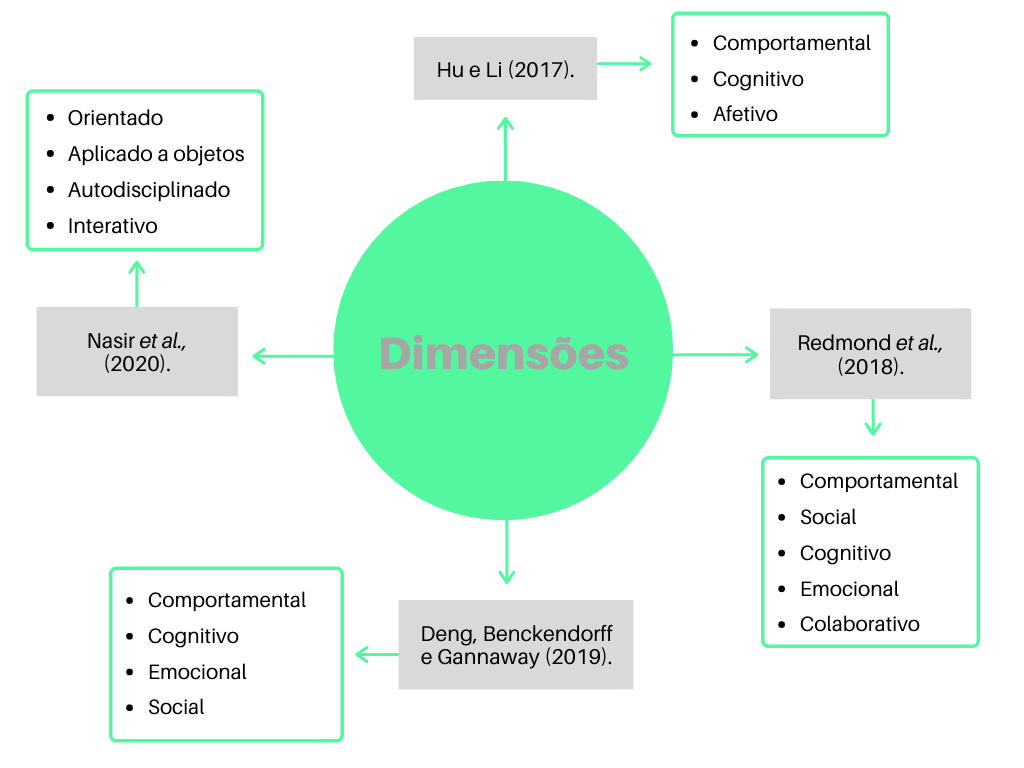
\includegraphics[width=0.85\textwidth]{fig1-35747.png}
 \caption{Dimensões do engajamento \textit{online}.}
 \label{fig1}
 \source{Elaboração própria (2021).}
\end{figure}

Há pouca unanimidade a respeito da definição de engajamento online na literatura. Autores mais recentes apontam diferentes dimensões para determiná-lo. O engajamento online pode incluir as três dimensões de engajamento já consagradas na literatura da área: comportamental, cognitivo e emocional. Existem condições individuais preditoras, influenciadas especialmente pela idade, motivação e habilidades \cite{hu2017}. Na literatura, encontram-se, também, cinco elementos de engajamento para o ensino e aprendizagem no ambiente online, tais como: social, comportamental, cognitivo, emocional e colaborativo. Tais elementos são considerados fundamentais para um estudante positivamente engajado e todos se relacionam entre si, determinando o padrão geral de engajamento em arranjos online \cite{redmond2018}.

Um estudo direcionado aos \emph{Massive Open Online Course} (MOOCs), conhecidos em português como Cursos Online Abertos e Massivos, conceitua o engajamento online como tendo quatro dimensões importantes: engajamento comportamental, cognitivo, emocional e social. Os recursos e os ambientes de aprendizagem online podem ser ajustados para atender às necessidades de distintos grupos de estudantes em cursos dessa natureza \cite{deng2020}. No estudo de \textcite{nasir2020}, o \emph{Student Course Engagement Questionnaire} (SCEQ) foi adaptado para ser aplicado em ambientes de ensino online. A adaptação, denominada SCEQ-M, possuindo quatro dimensões: engajamento aplicado, engajamento orientado a objetivos, engajamento autodisciplinado e engajamento interativo. Essa ferramenta pode ser útil em avaliações e pesquisas empenhadas em descobrir a estrutura e a força dos estilos de engajamento dos estudantes em cursos presenciais, online ou híbridos.

Essa síntese não exaustiva apresenta algumas possibilidades apresentadas na literatura a respeito de possíveis dimensões a serem consideradas quando o foco de um estudo é o engajamento online. Na sequência, será efetuado o detalhamento metodológico realizado para a revisão de escopo aqui proposta.

\section{Desenho metodológico}
Esta pesquisa se trata de uma revisão de escopo, tendo por finalidade identificar as metodologias empregadas na literatura internacional para mensurar o engajamento online de estudantes do ensino superior. Para a execução da pesquisa, seguimos o que sugere o modelo PRISMA-ScR para \emph{Scoping Review} \cite{tricco2018}. As revisões de escopo têm abordagem sistemática e servem para mapear traços ou indícios referentes a um determinado tópico, podendo explorar várias características, como alcance e natureza, e explorar como a pesquisa é dirigida em um campo específico \cite{tricco2018, peters2020}. Este estudo adota como \emph{framework} a estratégia PCC: População (P), Conceito (C) e Contexto (C) \cite{peters2020}. Os artigos selecionados para esta revisão possuem população (P) restrita a estudantes, quanto ao conceito (C), o engajamento online e o contexto (C), limitado ao ensino superior.

Dentre as diversas bases de dados disponíveis para pesquisas, optamos pela \emph{Dimensions} por se tratar de uma base que engloba muitas publicações, com uma amplitude vasta de dados, entre eles, artigos publicados em periódicos, pré-prints, livros e outros. Além disso, a \emph{Dimensions} possui indicadores baseados em citações e dados altimétricos, considerados como alternativos e mais democráticos em comparação às métricas tradicionais \cite{dimensions2021}. A escolha se deu também pelo fato de que ao realizarmos a pesquisa com a \emph{string} de busca definida para este estudo, o resultado da \emph{Dimensions} retornou dados mais precisos em relação às palavras-chave, comparados ao resultado da busca na \emph{Web of Science}, o que vai ao encontro do que assevera \textcite{thelwall2018}, quando aponta que o banco de dados da \emph{Dimensions} é uma opção emergente e eficaz em relação às concorrentes tradicionalmente mais prestigiadas, \emph{Scopus} e \emph{Web of Science}.

Considerando a pergunta central e o objetivo geral deste estudo, definimos os termos a serem pesquisados na base de dados: “online engagement”, “student engagement”, “higher education”, “instrument”, “scale” e “self-report”. Na \emph{string} de busca utilizamos os operadores \emph{booleanos} “AND” e “OR”. Os termos foram pesquisados em inglês por se tratar de uma busca que visa mapear as metodologias de mensuração do engajamento online de estudantes na literatura internacional. Entretanto, não foram incluídos filtros referentes a idiomas. A pesquisa foi realizada em 13 de maio de 2021 e considerou a busca na totalidade de cada documento e não apenas nos títulos, resumos ou palavras-chave. O período estabelecido para a busca foram os anos de 2017 a 2021 e foram incluídos os filtros para pesquisa somente de publicações que fossem artigos científicos e de acesso aberto.

Foram considerados para essa busca os últimos cinco anos, pelo fato desta revisão de escopo estar focalizada em uma literatura mais atual e também pelo fato de que publicações que abordam o conceito “online engagement” vêm crescendo. Quanto à seleção restrita a artigos e somente aqueles de acesso aberto, justificamos a escolha porque os artigos publicados em periódicos são consideradas publicações mais qualificadas e mais acessível do que a literatura cinzenta, a qual não possui numeração internacional padronizada e sua difusão é restrita \cite{botelho2002}. Já a opção pela seleção de artigos de acesso aberto se dá pela opção deliberada em defesa da difusão do conhecimento científico de fato mais acessível e democrático. A quantidade de documentos obtidos na base \emph{Dimensions} foi de 162 (cento e sessenta e dois). A \Cref{tab1} apresenta a \emph{string} de busca empregada.

\begin{table}[htpb]
\caption{\emph{String} de busca com os operadores \emph{booleanos}.}
\label{tab1}
\centering
\begin{tabular}{p{0.15\textwidth}p{0.75\textwidth}}
\toprule 
Base de dados & \emph{String} de busca
\\
\midrule
Dimensions &
Criteria: Text - '"online engagement" AND "student engagement" AND "higher education" and "instrument" OR "scale" OR "self-report" ' in full data; Publication Year is 2021 or 2020 or 2019 or 2018 or 2017; Publication Type is Article; Open Access is All OA.
\\ 
\bottomrule
\end{tabular}
\source{Elaboração própria (2021).}
\end{table}

Realizado o levantamento dos dados, o arquivo foi descarregado da base de dados e armazenado em uma planilha eletrônica do Google Docs. Os 162 registros identificados, seguindo o sugerido pelo Diagrama Prisma, passaram por uma análise inicial e oito itens foram excluídos antes da triagem por não se tratar de artigos ou não se referirem a artigos completos. A triagem que iniciou considerando 154 registros foi realizada em três etapas, que auxiliaram na seleção dos artigos potencialmente relevantes para esta revisão. As etapas consideraram, nesta ordem, a leitura de título e resumos, a leitura do artigo na íntegra e a leitura de artigo citado nos registros obtidos e incluídos na revisão posteriormente. Descrevemos a seguir os detalhes de cada uma das etapas:

Etapa 1: A estratégia de seleção compreendeu inicialmente a leitura dos títulos e resumos dos artigos, a fim de aplicar os critérios de inclusão e exclusão definidos para esta etapa. Os critérios de inclusão atenderam o seguinte: a) Artigo de pesquisa empírica; b) Tema central do artigo é engajamento \textit{online}; c) População pesquisada são estudantes; d) Contexto do artigo é ensino superior. Quanto aos critérios de exclusão, limitamos os seguintes: a) Artigo de revisão; b) Tema central do artigo não é engajamento \textit{online}; c) População pesquisada não são estudantes; d) Contexto do artigo não é ensino superior. Após a aplicação dos critérios descritos, foram selecionados 27 artigos e excluídos desta revisão, o total de 127 artigos.

O critério de exclusão (a) foi aplicado, considerando que artigos de revisão não possuem o escopo de mensurar ou construir uma estrutura de mensuração para reunir dados de um determinado grupo. Assim sendo, os itens excluídos por esse critério não contribuiriam para o alcance da resposta da pergunta central. Além disso, esta pesquisa tem o propósito de buscar os instrumentos para mensurar o engajamento \textit{online} de estudantes no ensino superior, logo, os critérios de exclusão (b), (c) e (d) visam limitar o levantamento de dados a estudos relacionados somente a esse tema, essa população e esse contexto, em consonância com a estratégia PCC adotada.

Etapa 2: esta etapa foi executada com base na leitura dos artigos em sua integralidade e os critérios de inclusão e exclusão se debruçaram na pergunta central deste artigo. Como critério de inclusão, definimos: (a) Artigo apresenta ou menciona questionário de mensuração de engajamento \textit{online}. Como critério de exclusão definimos: (a) Artigo não apresenta e não menciona questionário de mensuração de engajamento \textit{online}. O critério de inclusão se justifica pelo simples fato de que os artigos que não o atendem também não atenderão o escopo deste estudo. Nesta etapa, após a aplicação dos critérios, foram excluídos 18 artigos e mantidos nove artigos.

Etapa 3: A última etapa consistiu na inclusão dos artigos citados pelos estudos incluídos na etapa anterior, conforme parte do critério de inclusão (a) “menciona questionário de mensuração de engajamento online”. Nominamos os artigos incluídos por esse critério, como “artigos secundários”. Dos nove artigos incluídos na etapa anterior, quatro deles mencionaram questionário. Contudo, foram incluídos dois estudos secundários a esta revisão, em virtude de 2 dos estudos primários mencionarem o mesmo instrumento e um terceiro mencionar um instrumento construído pelo próprio autor em trabalho anterior. As etapas descritas até a obtenção da amostra final são apresentadas na \Cref{fig2}.

\begin{figure}[h!]
 \centering
 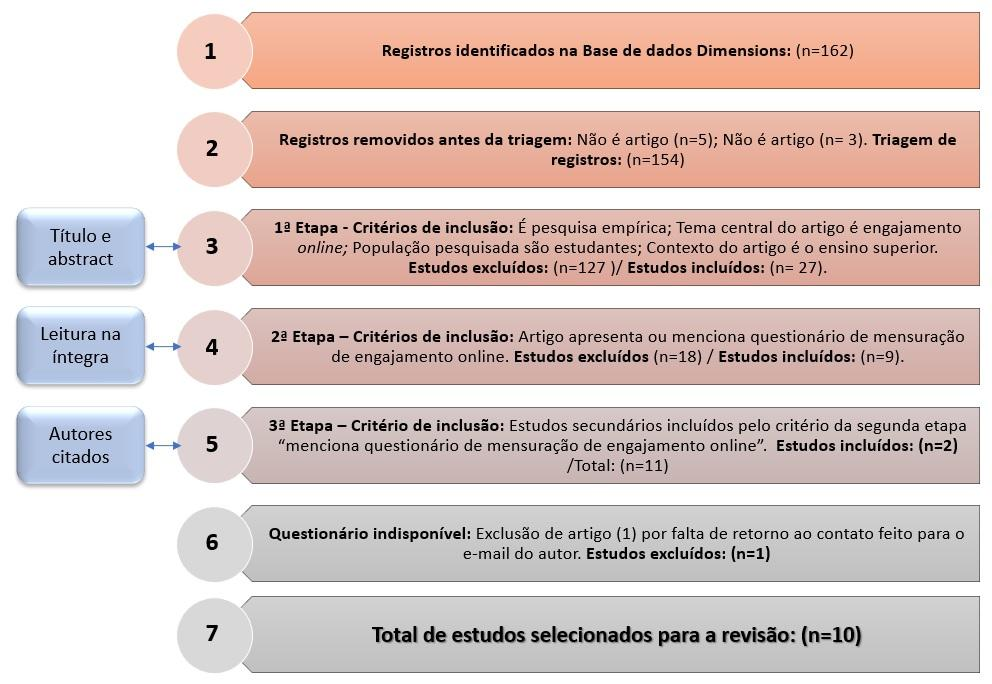
\includegraphics[width=0.9\textwidth]{fig2-35747.png}
 \caption{Processo de inclusão de artigos e amostra final.}
 \label{fig2}
 \source{Elaboração própria (2021).}
\end{figure}

Após a aplicação de todos os critérios definidos nas três etapas, o total de estudos incluídos nesta revisão de escopo foram 11, sendo a amostra composta por nove artigos incluídos através da base de dados \emph{Dimensions} e dois artigos inseridos secundariamente. Dois dos estudos selecionados, os quais traziam escalas construídas pelos autores, não apresentaram os instrumentos no artigo. Assim sendo, foi necessário contatar os autores através do e-mail disponibilizado nos artigos, de modo a obter as escalas para esta análise. Dos dois contatos realizados, recebemos retorno de apenas um deles. Dessa forma, foi necessário excluir desta revisão o artigo a respeito do qual não conseguimos acesso à informação fundamental para esta revisão: a escala de engajamento \textit{online}.

Após essa última exclusão, o total de dez estudos foram qualificados para a revisão. Os dados dos dez artigos incluídos foram organizados em uma nova planilha eletrônica do Google Docs e, de cada estudo, foram extraídos os seguintes aspectos: ano de publicação, idioma, país de publicação, autor(es), palavras-chave, objetivo do estudo, população pesquisada, metodologia utilizada e principais resultados. Na \Cref{tab2}, apresentamos a lista de artigos selecionados para análise.

%\begin{table}[h!]
\begin{longtable}{p{0.03\textwidth}p{0.87\textwidth}}
\caption{\emph{String} de busca com os operadores \emph{booleanos}.}
\label{tab2}
%\centering
\small
%\begin{tabular}{p{0.03\textwidth}p{0.87\textwidth}}
\\
\toprule 
ID & Referência do artigo
\\
\midrule
1 & HEIDARI, Elham et al. The role of digital informal learning in the relationship between students’ digital competence and academic engagement during the COVID‐19 pandemic. \textit{Journal of Computer Assisted Learning}, [s. l.], p. 1–13, 2021.
\\
2 & SHAH, Sobia Shafaq et al. Aprendizaje en línea durante la pandemia de COVID-19: aplicación de la teoría de la autodeterminación en la “nueva normalidad”. \textit{Revista de Psicodidáctica}, v. 26, n. 1, p.1–10,  2021.
\\
3 & WALKER, Kristen; KORALESKY, Katherine. \textit{Student and instructor perceptions of engagement after the rapid online transition of teaching due to COVID-19}. Natural Sciences Education, v. 50, n. 1, p. 1-10, 2021.
\\
4 & LUAN, Lin et al. Exploring the role of online EFL learners’ perceived social support in their learning engagement: a structural equation model. \textit{Interactive Learning Environments}, [s. l.], p. 1–12, 2020.
\\
5 & RAJABALEE, Yousra Banoor; SANTALLY, Mohammad Issack. \textit{Learner satisfaction, engagement and performances in an online module: Implications for institutional e-learning policy}. Education and Information Technologies, [s. l.], v. 26, n. 3, p. 2623–2656, 2021.
\\
6 & ERGÜN, Esin; KURNAZ ADIBATMAZ, Fatma Betül. Exploring the Predictive Role of E-Learning Readiness and E-Learning Style on Student Engagement. \textit{Open Praxis}, [s. l.], v. 12, n. 2, p. 175, 2020.
\\
7 & PICKERING, James D.; SWINNERTON, Bronwen J. \textit{Exploring the Dimensions of Medical Student Engagement with Technology-Enhanced Learning Resources and Assessing the Impact on Assessment Outcomes}. Anatomical Sciences Education, [s. l.], v. 12, n. 2, p. 117–128, 2019.
\\
8 & PYE, Graeme; HOLT, Dale; SALZMAN, Scott. Investigating different patterns of student engagement with blended learning environments in Australian business education: Implications for design and practice. \textit{Australasian Journal of Information Systems}, [s. l.], v. 22, 2018.
\\
9 & DIXSON, Marcia D. Measuring Student Engagement in the Online Course: The Online Student Engagement Scale (OSE). \textit{Online Learning}, [s. l.], v. 19, n. 4, 2015.
\\
10 & SUN, Jerry Chih-Yuan; RUEDA, Robert. Situational interest, computer self-efficacy and self-regulation: Their impact on student engagement in distance education: Student engagement in distance education. \textit{British Journal of Educational Technology}, [s. l.], v. 43, n. 2, p. 191–204, 2012.
\\ 
\bottomrule
%\end{tabular}
\source{Elaboração própria (2021).}
\end{longtable}
%\end{table}

Na seção seguinte (\ref{sec4}), serão descritos os dados observados nos artigos selecionados, bem como o contexto das pesquisas (universidade e país), objetivo dos estudos, quais os construtos avaliados nos questionários utilizados pelos autores, as dimensões e indicadores abordados nos instrumentos de mensuração de engajamento \textit{online}, os métodos de análise de dados utilizados e, ainda, buscaremos estabelecer comparações entre os instrumentos.

\section{Apresentação e análise dos dados}\label{sec4}
Iniciamos evidenciando os termos presentes nos títulos e \emph{keywords} dos artigos. Para isso, criamos manualmente uma nuvem de palavras com o auxílio da plataforma Mentimeter. Observamos uma grande diversidade de vocábulos, o que se justifica pelo fato de os estudos estarem dialogando com outros conceitos além do engajamento do aluno/estudante. A \Cref{fig3} demonstra os vocábulos que mais aparecem nos trabalhos investigados. Convém destacar que o termo que apresenta maior relevância conforme o resultado da figura é “engajamento do aluno”. Em ordem de frequência e destaque, seguem os demais termos: aprendizagem \textit{online}, ensino superior, engajamento dos alunos, Covid-19 e engajamento.

\begin{figure}[htbp]
 \centering
 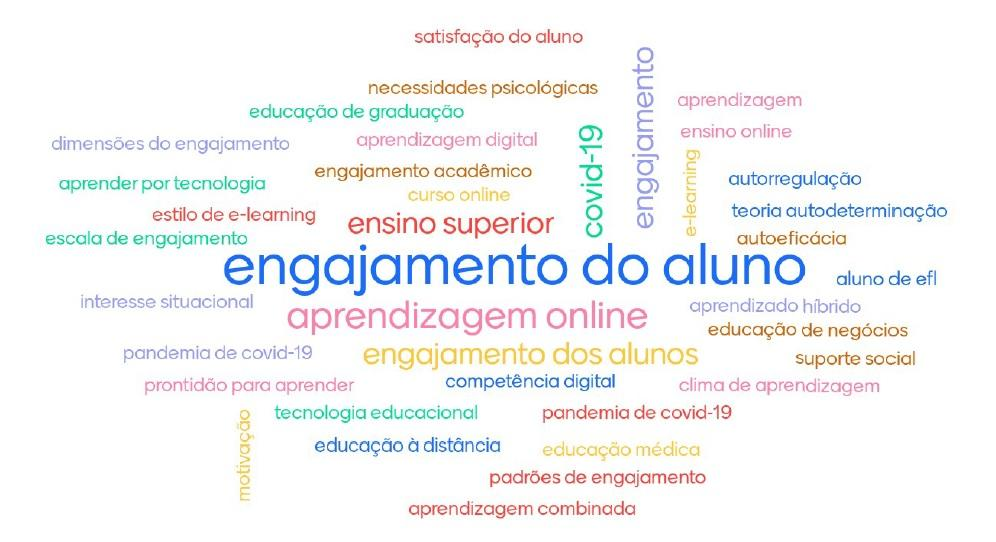
\includegraphics[width=0.90\textwidth]{fig3-35747.png}
 \caption{Nuvem de palavras dos títulos e \emph{keywords}.}
 \label{fig3}
 \source{Elaboração própria (2021).}
\end{figure}

Na \Cref{tab3}, são apresentados os dados iniciais da análise dos estudos. O período selecionado para o levantamento dos dados de publicação, conforme a string de busca, compreende os anos 2017 a 2021 (até maio), tendo um maior percentual (60\%) de publicações nos últimos dois anos: quatro artigos publicados em 2021 e dois em 2020. Os artigos são oriundos de nove países, apresentando baixa concentração de representatividade. Quanto aos idiomas, foram escritos somente em espanhol (n=1) e inglês (n=9). As áreas do conhecimento dos artigos, a partir dos três grandes colégios da CAPES, tomando como base os periódicos em que os estudos foram publicados e os enfoques de estudo, se concentram majoritariamente no Colégio de Ciências Exatas, Tecnológicas e Multidisciplinar.  

\begin{scriptsize}
%\begin{table}[ptbh]
\begin{longtable}{p{0.01\textwidth}p{0.1\textwidth}p{0.19\textwidth}p{0.10\textwidth}p{0.08\textwidth}p{0.16\textwidth}p{0.16\textwidth}}
\caption{Características iniciais dos artigos revisados.}
\label{tab3}
%\begin{tabular}{p{0.01\textwidth}p{0.1\textwidth}p{0.17\textwidth}p{0.1\textwidth}p{0.08\textwidth}p{0.15\textwidth}p{0.2\textwidth}}
\\
\toprule 
ID & Autoria & Instituição dos autores & País de origem da pesquisa & Idioma & Periódico de publicação & Área do conhecimento
\\
\midrule
1 & \textcite{heidari2021} & Shiraz University e Open University of the Netherlands & Irã & Inglês & \emph{Journal of Computer Assisted Learning} & Colégio de Ciências Exatas, Tecnológicas e Multidisciplinar
\\
2 & \textcite{shah2021} & University of Sindh;
Mehran University of Engineering and Technology; University of Essex. & Paquistão & Espanhol & \textit{Revista de Psicodidáctica} &
Colégio de Humanidades
\\
3 & \textcite{walker2021} & University of British Columbia & Canadá & Inglês & \textit{Natural Sciences Education} & Colégio de Ciências da Vida
\\
4 & \textcite{luan2020} & Beijing Normal University; National Taiwan Normal University; Shandong Normal University;
Central China Normal University. & China & Inglês & \textit{Interactive Learning Environments} & Colégio de Ciências Exatas, Tecnológicas e Multidisciplinar
\\
5 & \textcite{rajabalee2021} & Mauritius Institute of Education;
University of Mauritius Reduit. & Maurícia & Inglês & \textit{Education and Information Technologies} & Colégio de Ciências Exatas, Tecnológicas e Multidisciplinar
\\
6 & \textcite{ergun2020} & Karabuk University. & Turquia & Inglês & \textit{Open Praxis} & Colégio de Ciências Exatas, Tecnológicas e Multidisciplinar
\\
7 & \textcite{pickering2019} & University of Leeds. & Reino Unido & Inglês & \textit{Anatomical Sciences Education} & Colégio de Ciências da Vida
\\
8 & \textcite{pye2018} & Deakin University. & Austrália & Inglês & \textit{Australasian Journal of Information Systems} & Colégio de Ciências Exatas, Tecnológicas e Multidisciplinar
\\
9 & \textcite{dixson2015} & Indiana University – Purdue University Fort Wayne. & Estados Unidos & Inglês & \textit{Online Learning} & Colégio de Ciências Exatas, Tecnológicas e Multidisciplinar
\\
10 & \textcite{sun2012} & National Chiao Tung University;
University of Southern California. & Estados Unidos & Inglês & \textit{British Journal of Educational Technology} & Colégio de Ciências Exatas, Tecnológicas e Multidisciplinar
\\ 
\bottomrule
%\end{tabular}
\source{Elaboração própria (2021).}
%\end{table}
\end{longtable}
\end{scriptsize}

Quanto ao contexto, quatro desses trabalhos foram realizados durante a pandemia de Covid-19. Em relação às amostras, foram compostas predominantemente de estudantes, tendo apenas um dos estudos envolvido, além de estudantes, instrutores da universidade. Pode-se observar ainda, que apresentam uma variação em relação ao tamanho da amostra, sendo a maior composta por 689 pessoas e a menor por 34 pessoas. Em relação ao objetivo e foco das pesquisas, na maioria dos artigos revisados, o conceito de engajamento dialoga com outros conceitos, visando observar se há associação entre eles. Apenas três dos estudos tratam unicamente do engajamento (ID: 3, 8 e 9), sem fazer associações com outros construtos. Quanto à metodologia, observa-se que a característica principal dos artigos revisados é que utilizam delineamentos quantitativos, apenas dois deles de métodos mistos (ID: 3 e 5). Os dez estudos coletaram dados através de questionários e realizaram análises diversificadas, pormenorizadas na \Cref{tab4}, sendo mais frequentes a modelagem de equações estruturais e os testes de correlação.

\begin{small}
\begin{longtable}{p{0.01\textwidth}p{0.2\textwidth}p{0.12\textwidth}p{0.23\textwidth}p{0.29\textwidth}
    }
\caption{Contexto, população, objetivo/foco e metodologia dos artigos revisados.}
\label{tab4}
\\
\toprule
ID & Contexto & População pesquisada & Objetivo e foco & Metodologia
\\
\midrule
1 & O estudo foi realizado com estudantes da Universidade de Shiraz, Irã, durante a pandemia de Covid-19. & A amostra do estudo incluiu 308 alunos. & O estudo tem como objetivo investigar se havia uma relação significativa entre a aprendizagem digital informal, as competências digitais dos alunos e seu engajamento acadêmico. & Estudo quantitativo com levantamento de dados através de questionários enviados aos alunos. Os dados foram analisados por meio de modelagem de equações estruturais e análises descritivas utilizando o software SPSS.
\\
\arrayrulecolor{gray}
\midrule
2 & Estudantes que participaram de aulas \textit{online} em dez universidades  do Paquistão (cinco públicas e cinco privadas) durante a pandemia de Covid-19. & A amostra compreendeu 689 alunos. & O estudo investiga a fundo a transição efetiva para o “novo normal” do ensino a distância e o papel mediador das necessidades psicológicas básicas dos alunos no nexo entre o clima de aprendizagem virtual e o engajamento do aluno. & Estudo de cunho quantitativo, em que os participantes responderam a uma pesquisa \textit{online}, através de questionário. Para a análise dos dados realizou-se a modelagem de equações estruturais com o SPSS.
\\
\midrule
3 & Alunos de graduação e instrutores de quinze cursos em uma grande universidade canadense durante a pandemia de Covid-19. & A pesquisa foi realizada com 11 instrutores e 145 alunos. & Este estudo avaliou as percepções de alunos de graduação e instrutores sobre os componentes inter-relacionados de engajamento durante e após a rápida transição \textit{online} de ensino em março de 2020, devido à pandemia Covid-19. & Estudo de métodos mistos, em que pesquisas com instrutores e pesquisas com alunos foram administradas. Os alunos foram apresentados a escalas quantitativas Likert e perguntas abertas qualitativas. As respostas da pesquisa foram baixadas e organizadas em Microsoft Excel.
Os valores medianos foram calculados para o conjunto de respostas em escala Likert.
Para as perguntas abertas, foi utilizada a análise de conteúdo dirigida.
\\
\midrule
4 & Estudantes universitários da China durante a pandemia de Covid-19. & Um total de 615 estudantes universitários da China foram convidados a participar do estudo. & O estudo tem o objetivo de explorar se o suporte social percebido pelos alunos de \emph{English as a foreign language} (EFL) online promoveria ou dificultaria seu engajamento na aprendizagem online. & Este estudo é de cunho quantitativo e utilizou questionários para o levantamento dos dados. A modelagem de equações estruturais foi realizada para fornecer uma medição mais precisa das relações de estrutura entre todos os construtos. Com base na modelagem de equações estruturais, os efeitos mediacionais foram testados usando o procedimento AMOS \emph{bootstrap}.
\\
\midrule
5 & Estudantes universitários no primeiro ano do ensino nacional da Maurícia em diferentes disciplinas: Engenharia, Ciências, Humanidades, Gestão e Agricultura.& A amostra foi composta de 665 alunos da universidade. & O estudo investigou as relações entre o engajamento dos alunos, seus níveis de satisfação e seus desempenhos gerais em um módulo \textit{online}. & Esta pesquisa utilizou uma abordagem de método misto. O método primário foi a coleta e análise quantitativa de dados por meio de medidas do grau de associação entre as variáveis e os dados qualitativos foram levantados por meio do feedback dos alunos através de um questionário de perguntas abertas. A análise da etapa quantitativa focou principalmente em estatísticas aplicadas, como testes t e testes de correlação. Para a etapa qualitativa foi realizada análise de conteúdo.
\\
\midrule
6 & Alunos do Centro de Educação a Distância da Universidade pública de Karabuk na Turquia que fizeram o curso de Medição e Avaliação em Educação durante o ano letivo de 2016–2017. & A amostra contou com 527 alunos do último ano. & O objetivo deste estudo foi determinar os fatores que predizem o engajamento dos alunos. &
Esta pesquisa tem abordagem quantitativa. Na coleta de dados, foi aplicado um questionário. A análise de regressão múltipla \emph{stepwise} foi usada para analisar os dados.
\\
\midrule
7 & Estudantes de medicina do primeiro ano do componente de anatomia integrada do programa \emph{Bachelor of Medicine} e \emph{Bachelor of Surgery} na University of Leeds, Reino Unido. & Foi realizada com 192 estudantes de medicina. & Este estudo tenta investigar as dimensões do engajamento dos alunos com recursos de aprendizagem aprimorados pela tecnologia como parte do currículo de anatomia de um programa médico. & Este estudo é de natureza quantitativa. Foi aplicado um questionário para levantamento dos dados. A análise foi realizada através de estatísticas descritivas. Todos os dados foram classificados, codificados e analisados usando o software SPSS.
\\
\midrule
8 & Alunos de graduação do programa de comércio de uma universidade australiana. & A amostra foi composta por 138 alunos no primeiro trimestre e 42 alunos no segundo trimestre. & A pesquisa se estende ao trabalho realizado sobre o engajamento dos alunos em ambientes \textit{online} e reside no domínio do design e da prática de aprendizagem combinada no contexto empresarial australiano de ensino superior. & Este estudo é de caráter quantitativo. O levantamento de dados foi realizado através de um questionário já validado pela literatura. Os dados foram gerenciados usando Microsoft XL 2013 e analisados usando XL Statistics. O teste Qui-quadrado de Pearson foi usado para testar se dois conjuntos de dados categóricos eram independentes. Para avaliar as diferenças entre duas médias, o teste t foi usado.
\\
\midrule
9 & Alunos de 5 cursos de comunicação \textit{online} de nível superior em um centro-oeste regional universitário dos EUA. & A pesquisa foi respondida por 34 alunos. & Este estudo fornece validação da escala de engajamento do aluno \textit{online}, correlacionando os autorrelatos do aluno sobre o engajamento com dados de rastreamento do comportamento do aluno a partir de um sistema de gerenciamento de curso \textit{online}. & Esta pesquisa é de natureza quantitativa. O levantamento dos dados foi realizado através de questionário e rastreamento de informações sobre comportamentos de aprendizagem dos alunos. Os resultados foram analisados executando correlações de Pearson entre o questionário e o número de comportamentos de aprendizagem.
\\
\midrule
10 & Estudantes de graduação do semestre de outono de 2008 nas Escolas de Gerontologia e Engenharia, matriculados em aulas \textit{online}, em uma grande universidade de pesquisa no sudoeste dos EUA. & Os participantes foram 203 alunos. & 
Este estudo investiga possíveis relações entre variáveis motivacionais e de aprendizagem (interesse, autoeficácia e autorregulação) e três tipos de engajamento do aluno (comportamental, emocional e cognitivo) em um ambiente de educação a distância. & 
Este estudo é de caráter quantitativo. Os dados foram levantados através de questionários adaptados de escalas validadas existentes. Foram realizadas análise de intercorrelações e análises de regressão hierárquica.
\\
\arrayrulecolor{black}
\bottomrule
\source{Texto de preenchimento gerado pelo pacote lipsum.}
\end{longtable}
\end{small}

Em relação às características dos questionários utilizados nos estudos, apresentadas na \Cref{tab5}, observamos que em sete artigos (ID: 1, 2, 4, 5, 6, 7 e 10) são avaliados mais de um construto. Desses sete, cinco utilizam questionários distintos de perguntas fechadas para analisar cada construto e dois (ID: 5 e 7) utilizam, respectivamente, um questionário de perguntas abertas e um questionário de perguntas fechadas único, elaborados para analisar todos os construtos. Três dos estudos (ID: 3, 8 e 9) utilizam questionários de perguntas fechadas que avaliam apenas o construto de engajamento. Analisando exclusivamente os questionários que avaliam o engajamento, foco desta revisão, observamos que sete são explicitamente de escala Likert de cinco pontos, com respostas que em sua maioria possuem redação “concordo totalmente” e “discordo totalmente”. Dois dos artigos que utilizam questionários de perguntas fechadas não explicitam o tipo de escala e redação (ID: 6 e 8). Os questionários variam entre 17 e 30 itens, contudo estão em maior número os que possuem entre 17 e 19 itens (ID: 1, 2, 6, 7, 9, 10). Os questionários que avaliam o engajamento do aluno e o subdividem em dimensões (ID: 1, 2, 3, 4, 6, 9, 10), consideram entre três e quatro dimensões, com exceção do ID: 3, que considera apenas duas. Entre as dimensões consagradas pela literatura, mencionadas anteriormente, as dimensões mais frequentemente consideradas nos artigos desta revisão são: engajamento comportamental, engajamento emocional/afetivo e engajamento cognitivo.

\begin{small}
\begin{longtable}{p{0.01\textwidth}p{0.18\textwidth}p{0.18\textwidth}p{0.18\textwidth}p{0.15\textwidth}p{0.18\textwidth}
    }
\caption{Contexto, população, objetivo/foco e metodologia dos artigos revisados.}
\label{tab5}
\\
\toprule
ID & Construtos avaliados no artigo & Dimensões/ Indicadores/Fatores avaliados & Tipo de questionário e redação & Fonte ou base para a construção do questionário & Natureza das questões

\\
\midrule
1 & A pesquisa avalia os construtos de engajamento acadêmico, competência digital e \emph{digital informal learning} (DIL). Para isso, utilizou três escalas distintas, uma delas a Escala de Engajamento Acadêmico. &
A Escala de Engajamento Acadêmico possui 17 itens, distribuídos em três dimensões: vigor, absorção e dedicação. &
A escala é  Likert de 5 pontos, onde: (1 = discordo totalmente; 5 = concordo totalmente). & 
A Escala de Engajamento acadêmico desenvolvida é uma versão abreviada da \emph{Utrecht work engagement scale} \cite{schaufeli2006}. &
Os itens do questionário de Engajamento Acadêmico presentes na escala não são voltados para contextos \textit{online}. Estão mais direcionados a identificar o quanto o aluno está envolvido com seu campo de estudo especificamente.
\\
\arrayrulecolor{gray}
\midrule
2 & O estudo analisa os construtos clima de aprendizagem, necessidades psicológicas básicas e motivação dos estudantes. Para isso, utilizou três escalas, uma delas a \emph{Online Student Engagement} (OSE). &
A \emph{Online Student Engagement Scale} possui 18 itens distribuídos em quatro dimensões: habilidades, emoções, participação e desempenho. &
A escala é Likert de 5 pontos, onde: (1 = discordo totalmente; 5 = concordo totalmente). &
A escala adotada foi a Online Student Engagement (OSE); \cite{dixson2015} &
A escala se aplica ao contexto do ensino \textit{online}, entretanto o questionário traz itens que medem situações em que é utilizado especificamente o recurso de fóruns \textit{online}.
\\
\midrule
3 & A pesquisa trata somente do engajamento dos estudantes. Para isso foi elaborado um questionário de perguntas fechadas com base em Prompts de atividades que aborda os engajamentos cognitivo e afetivo e, além disso, um conjunto de perguntas abertas sobre engajamento comportamental. & O questionário de perguntas fechadas possui 29 itens que avaliam duas dimensões: engajamento cognitivo e afetivo. Possui questões relacionadas aos seguintes prompts de atividade: Ensino síncrono, Ensino assíncrono, Preparação do aluno, Engajamento dos colegas, Avaliação, Laboratório. & As respostas foram coletadas usando uma escala Likert de 5 pontos, sendo 1 = muito envolvente, 2 = envolvente, 3 = neutro, 4 = um pouco envolvente, 5 = não envolvente. & O questionário se baseia em Prompts de atividade apresentados aos alunos para avaliar o quão engajante um aluno encontraria uma determinada atividade se eles fizessem o mesmo curso novamente em um ambiente totalmente \textit{online}. & As atividades de prompt sugeridas para avaliar as dimensões se aplicam ao contexto do ensino \textit{online}, exceto o último grupo, que traz questões relacionadas a atividades de laboratório.

\\
\midrule
4 & O estudo avalia os construtos de apoio social no contexto da aprendizagem \textit{online} (apoio de professor, apoio de pares) e engajamento do aluno no contexto da aprendizagem \textit{online}. Para isso, utiliza duas escalas, entre elas a \emph{Online English Learning Engagement} (OELE). & 
A escala possui 20 itens que avaliam quatro dimensões de engajamento: Engajamento comportamental,
Engajamento cognitivo,
Engajamento emocional,
Engajamento social. & 
A escala é Likert de 5 pontos, onde: (1 = discordo totalmente; 5 = concordo totalmente). & O questionário OELE foi adaptado da medida desenvolvida por \textcite{wang2021}. & As questões são todas direcionadas ao contexto de aulas de Inglês, ademais o questionário possui apenas uma questão que menciona o ambiente online.
\\
\midrule
5 & A pesquisa analisa os construtos desempenho, satisfação e engajamento dos alunos em cursos online. Para isso, desenvolveu os \emph{Student Feedback questionnaire}. & O questionário possui 27 itens que avaliam os construtos de satisfação e engajamento dos alunos. São 5 grupos de questões que possuem entre 5 e 6 questões cada. & O questionário é composto por perguntas abertas que abordam os construtos de satisfação e engajamento dos alunos em cursos \textit{online}. O artigo não traz conceitos de dimensões de engajamento. & Construído a partir do \emph{Online Student Engagement} (OSE), \textcite{dixson2015} e \emph{Online Learning Consortium}. & As questões presentes no questionário podem ser aplicadas ao contexto de graduação em ambiente \textit{online}, contudo o questionário avalia outros construtos além do engajamento.
\\
\midrule
6 & A pesquisa avalia os construtos engajamento do aluno, estilo de \emph{e-learning} e a prontidão para o aprendizado \textit{online}. Para isso, foram utilizadas três escalas, uma delas a \emph{Engagement Scale}. & A escala possui 19 itens que avaliam as dimensões de engajamento comportamental, engajamento afetivo e engajamento cognitivo. & Os autores não detalham o tipo de \emph{Likert} da Escala de engajamento do aluno, tampouco sua redação. Originalmente a escala é \emph{Likert} de 5 pontos, onde: 5 = concordo totalmente, 4 = concordo, 3 = não concordo nem discordo, 2 = discordo e 1 = discordo totalmente. Contudo, isso não é pormenorizado no artigo. &
Foi utilizada a Escala validada \emph{Engagement Scale} \cite{sun2012}. & A \emph{Engagement Scale} \cite{sun2012} possui questões direcionadas ao contexto online e ensino superior. Possui questões como "Quando estou na aula online, apenas "ajo" como se estivesse aprendendo." e "Gosto de fazer as aulas online".
\\
\midrule
7 & O estudo analisa os construtos de engajamento do aluno e tecnologia-enhanced learning (TEL). Para isso, utilizou a \emph{Technology-enhanced learning} (TEL) \emph{engagement instrument}. & A pesquisa de engajamento TEL usada neste estudo consiste em uma escala final de 19 itens que avalia três fatores emergentes: satisfação, definição de metas e planejamento e interação física. & A escala é Likert de cinco pontos: Discordo totalmente= 1; discordo= 2; nem concordo nem discordo= 3; concordo= 4; concordo totalmente= 5. & A escala foi construída com base: (1) a escala de motivação e aprendizagem autorregulada \cite{fontana2015, milligan2016}, (2) a escala de engajamento online \cite{krause2008}, e
(3) a escala de envolvimento do aluno \cite{gunuc2015}. & As questões buscam averiguar o quanto os alunos gostam de utilizar recursos TEL  (Tecnologia para aprimorar a aprendizagem) em suas aulas. A escala não averígua especificamente aulas em ambientes online. Avalia a inclusão desses recursos. Ainda, a escala aborda outros dois construtos além do engajamento do aluno.
\\
\midrule
8 & O estudo analisa o engajamento do aluno em ambiente de aprendizagem híbrido. Para isso, desenvolveu o \emph{Online student engagement constructs for contemporary blended learning environments}. & A escala utilizada neste estudo consiste em 30 itens, divididos em sete fatores: aprendizagem ativa online, interação social online, colaboração online, ensino online, avaliação online, relevância acadêmica online e contato online com a equipe. & O artigo não menciona qual o tipo de escala utilizado, contudo, no texto das análises, as respostas se baseiam em manifestações de concordar ou não com as afirmações por parte dos respondentes, o que sugere a utilização de escala tipo Likert. & Baseia-se em uma escala de engajamento do aluno já desenvolvida, testada e validada relacionada à aprendizagem online por \cite{coates2016}. & As questões da escala envolvem em sua maioria o \emph{Cloud Deakin}, que é um ambiente de aprendizagem em nuvem e estão voltadas ao ensino híbrido, assim sendo, não se aplica ao contexto de cursos do ensino superior em geral.
\\
\midrule
9 & O artigo trata apenas do engajamento online, objetivando o desenvolvimento da escala de medição \emph{Online Student Engagement}. & A escala possui 19 itens que avaliam as dimensões: engajamento de habilidades, engajamento emocional, engajamento de participação/interação e engajamento de desempenho. &
A escala é Likert de 5 pontos: 1. nada característico de mim
2. não é realmente característico de mim
3. moderadamente característico de mim
4. característica de mim
5. muito característico de mim. & 
\textcite{handelsman2005} SCEQ foi usado para formar a base do \emph{Online Student Engagement}. & 
A escala se aplica ao contexto do ensino online, entretanto o questionário traz itens que medem situações em que é utilizado especificamente o recurso de fóruns online.
\\
\midrule
10 & O estudo avalia as variáveis motivacionais e de aprendizagem (interesse, autoeficácia e autorregulação) e o engajamento do aluno. Para isso, a pesquisa utilizou 4 escalas distintas, uma delas, a \emph{Engagement Scale}. & A escala de engajamento possui 19 itens distribuídos em três dimensões: engajamento comportamental, engajamento emocional e engajamento cognitivo. & A escala é Likert de 5 pontos, onde: 5 = concordo totalmente, 4 = concordo, 3 = não concordo nem discordo, 2 = discordo e 1 = discordo totalmente. & A Escala de Engajamento foi adaptada de \textcite{fredricks2004,fredricks2005}. & A Escala de Engajamento \cite{sun2012} possui questões direcionadas ao contexto online e ensino superior. Possui questões como "Quando estou na aula online, apenas "ajo" como se estivesse aprendendo." e "Gosto de fazer as aulas online".
\\
\arrayrulecolor{black}
\bottomrule
\source{Texto de preenchimento gerado pelo pacote lipsum.}
\end{longtable}
\end{small}

Quanto à fonte de referência ou base para a construção dos questionários utilizados nos artigos, apenas dois utilizam instrumentos já validados (ID: 2 e 6). Os demais utilizam questionários construídos ou adaptados de outros. Em relação à natureza das questões, observamos que quatro dos questionários (ID: 1, 4, 7 e 8) não se aplicam especificamente ao contexto geral do ensino superior de forma online, por terem questões direcionadas ao ensino de inglês, questões direcionadas a identificar o engajamento do aluno especificamente com seu campo de estudo, questões direcionadas a identificar o quanto os alunos gostam de utilizar recursos tecnológicos em suas aulas ou questões que analisam especificamente o uso de um ambiente de aprendizagem em nuvem particular.

Sintetizando, a maioria dos artigos possui abordagem quantitativa e todos eles utilizam algum tipo de questionário para a coleta de dados. Os questionários que avaliam o engajamento, utilizados nos artigos desta revisão de escopo são, em maioria, de perguntas fechadas e adotam escala Likert de 5 pontos, com redações que, em maior número, variam entre “concordo totalmente” e “discordo totalmente”.

Os questionários aplicados nas pesquisas limitam-se a um número de itens que varia entre 17 e 19. O número de dimensões de engajamento, dos questionários que possuem essa subdivisão, varia entre três e quatro e as dimensões mais frequentes são engajamento comportamental, engajamento emocional/afetivo e engajamento cognitivo. A técnica de análise mais presente nos artigos é a modelagem de equações estruturais, empregada em três pesquisas. Nos demais artigos aparecem a análise de conteúdo dirigida, análise de regressão múltipla stepwise, análises de regressão hierárquica, o teste Qui-quadrado de Pearson e correlações de Pearson.

\section{Considerações finais}
Para concluir, retomamos os aspectos mais relevantes encontrados nos artigos revisados. Um percentual significativo dos artigos foi publicado já no período de pandemia de Covid-19. Isso revela o interesse crescente da pesquisa educacional em compreender os processos de engajamento estudantil a partir das especificidades que configuram a aprendizagem online. São artigos de autores de nacionalidades diversas, havendo apenas dois de mesma origem, dos EUA. São pesquisas escritas mormente em inglês, o que corresponde a nove artigos de um total de dez. As amostras, compostas de estudantes de ensino superior, variam em número de respondentes, sendo a maior composta por 689 alunos e a menor 34 alunos. Na maioria dos artigos o construto de engajamento do aluno dialoga com outros conceitos, por exemplo, competência digital, clima de aprendizagem, autoeficácia e autorregulação. Vale dizer que, nesse diálogo, percebe-se a necessidade de uma maior compreensão, por parte de muitos pesquisadores, entre os limites e as especificidades de cada conceito, no intuito de efetivamente analisá-los sem ocorrência de sobreposições.

Dito isso, resgatamos nossa pergunta central de pesquisa, a fim de evidenciar as contestações: quais as características dos instrumentos e das técnicas analíticas utilizadas para a mensuração do engajamento online de estudantes do Ensino Superior em pesquisas publicadas recentemente (2017-2021) na literatura internacional? Os dados apresentados resumem tanto as características dos questionários, quanto as técnicas analíticas adotadas, o que responde, em parte, a nossa pergunta central. Contudo, a busca nesta revisão é por instrumentos que avaliam especificamente o engajamento online, o que de fato não se revela plenamente no escopo de todos os questionários analisados.

Há quatro questionários que, embora aplicados em ambientes online, não foram construídos para avaliar as especificidades desse contexto, já que possuem números insignificantes de questões focadas nesse ambiente. Há casos que tendem a buscar exclusivamente averiguar o quanto os alunos gostam de utilizar recursos de aprendizagem por tecnologia ou, ainda, envolvem questões que exploram apenas o uso de algum ambiente de aprendizagem específico.
Os questionários Prompts de atividade \cite{walker2021}, \emph{Student Feedback questionnaire} \cite{rajabalee2021}, \emph{Engagement Scale} \cite{sun2012} e \emph{Online Student Engagement} \cite{dixson2015} são os que possuem questões que se aplicam ao ensino online, entretanto, em relação aos dois primeiros, um avalia outros construtos além do engajamento e outro traz indagações que envolvem atividades de laboratório, o que não pode ser aplicado de maneira escalonável para  todos os alunos de graduação. O instrumento de \textcite{dixson2015} compreende a utilização de fóruns online, ferramenta que não é adotada por todas as universidades.

Podemos afirmar, como conclusão desta revisão de escopo, que dos dez instrumentos avaliados, unicamente o de \textcite{sun2012} pode ser utilizado para avaliar o engajamento online do estudante no contexto do ensino superior de forma escalonável, ou seja, estendida a qualquer curso, independentemente de suas características. Como sugestão para pesquisas futuras, indica-se a construção de uma nova escala específica para análise de engajamento online, que busque considerar mais aspectos vinculados às especificidades do contexto de aprendizagem online em comparação aos instrumentos aqui analisados, com perspectiva de adoção em grande escala em universidades brasileiras. Nessa perspectiva, ainda, sugere-se que possam ser estipuladas teoricamente as bases que justificam a definição de cada subconstruto adotado, especialmente considerando as características próprias dos ambientes online.

\printbibliography\label{sec-bib}
% if the text is not in Portuguese, it might be necessary to use the code below instead to print the correct ABNT abbreviations [s.n.], [s.l.]
%\begin{portuguese}
%\printbibliography[title={Bibliography}]
%\end{portuguese}


%full list: conceptualization,datacuration,formalanalysis,funding,investigation,methodology,projadm,resources,software,supervision,validation,visualization,writing,review
\begin{contributors}[sec-contributors]
\authorcontribution{Fernanda da Cunha Ortega}[datacuration,investigation,visualization,writing]
\authorcontribution{Valesca Brasil Irala
}[conceptualization,projadm,supervision,review]
\end{contributors}


\end{document}
